\section{Introduction}
\label{sec:intro}

%\KZ{Our premise: Review sentences tend to be short and informative. It is our belief
%that every sentence in a review should provide some useful info.}

Abstractive opinion summarization is the process of 
automatically producing a summary for a set of 
subjective user reviews given an entity 
(a place, a product, a service, et.al.). 
Such a set of reviews is called a {\em multi-review} in this paper. 
The deep learning (DL) techniques has made a great success 
in abstractive summarization
~\cite{NallapatiZSGX16,SeeLM17,LiuLZ18,CelikyilmazBHC18,BART20}, which need training on a large number of text-summary pairs.
Unfortunately, the opinion summarization task 
generally lacks the multi-review and reference summary pairs,
as it is difficult for annotators to write summaries for 
multi-reviews on a large scale.

\begin{figure}[th]
	\centering
	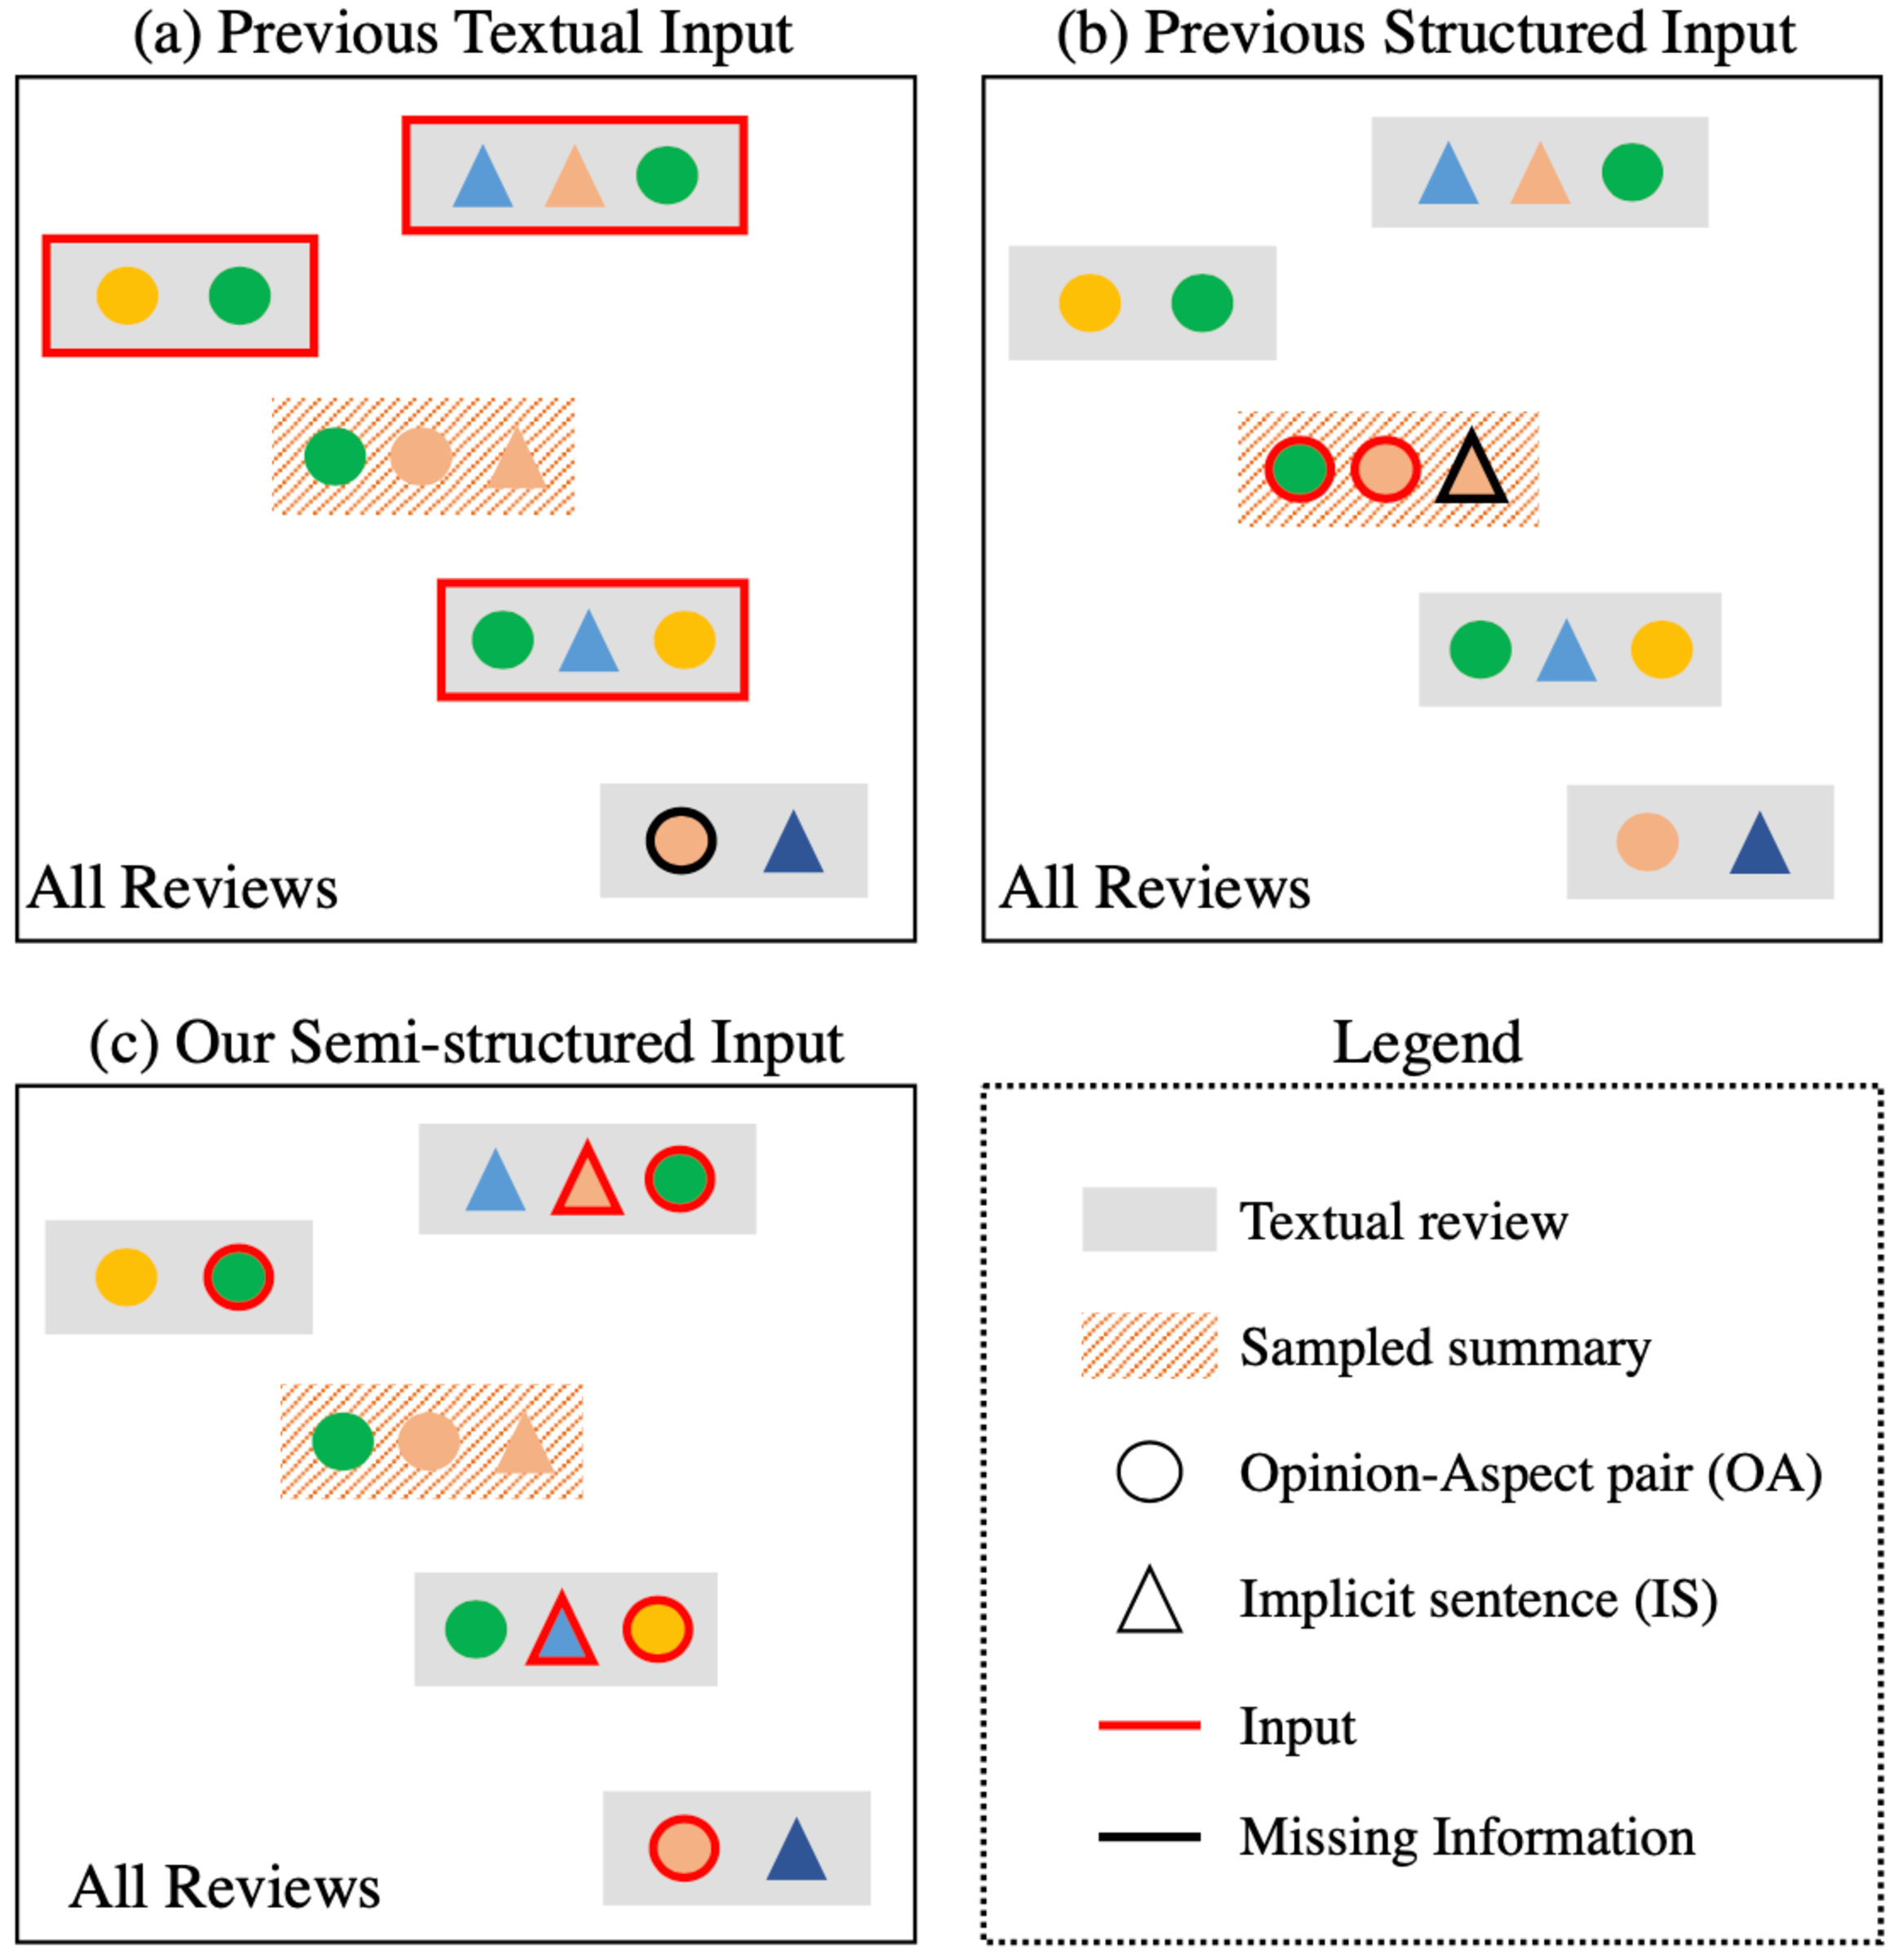
\includegraphics[width=0.85\linewidth]{./brief.pdf}
	\caption{Different synthetic inputs of the same summary.
	}
	\label{fig:brief}
\end{figure}
\begin{table}[th]
	\centering
	\scriptsize
	
	\begin{tabular}{|p{7.2cm}|}
		\hline \rule{0pt}{10pt}
		\makecell[c]{\bf Output (Sampled Summary)} \\
		\hline
		very \textbf{disappointed} in \textbf{food} and \textbf{service} . the \textbf{beef} was \textbf{burned} . 
		\underline{the \textbf{staff} \textbf{dismissed} my comments .}
		\vspace{0.2em}\\
		\hline
	\end{tabular}


	\begin{tabular}{|m{0.95cm}|m{0.3cm}<{\centering}|m{5.1cm}|}
	\hline
	\multicolumn{3}{|c|}{\rule{0pt}{10pt} \bf Input}  \\	
	\hline
	\multirow{3}{0.1cm}{FewSum} & $R_1$ & very average spanish \textbf{food} .
	\\
	\cline{2-3}
	& $R_2$ &definitely not a peruvian restaurant
.
	\\
	\cline{2-3}
	& $R_3$ &love this place! location is great
.
	\\
    \hline
	\multirow{3}{0.1cm}{Denoise} & $R_1$ & very uncomfortable in \textbf{food} and \textbf{staff} . the \textbf{ food} was bad . the \textbf{staff} ignored me .
	\\
	\cline{2-3}
	& $R_2$ & bad \textbf{food} . the \textbf{staff} ignored me . very uncomfortable in restaurant .\\
	\cline{2-3}
	& $R_3$ &I was \textbf{disappointed} with the restaurant. the \textbf{food} was not bad . but the \textbf{staff} was unfriendly .
	\\
	\hline
	\multirow{3}{0.1cm}{PlanSum} & $R_1$ & bad \textbf{food} and \textbf{service} . \textbf{disappointed} \\
	\cline{2-3}
	& $R_2$& the \textbf{food} and \textbf{service} was not good . very \textbf{bad experience} .
\\
	\cline{2-3}
	& $R_3$ &awful \textbf{food} and \textbf{service} . the \textbf{staff} was unfriendly .
	\\
	\hline
	OpiDig & OA & \textbf{disappointed}, \textbf{food; disappointed}, \textbf{service; burned}, \textbf{beef}
	\\
	\hline
	\multirow{2}{0.1cm}{Ours} & OA &not good, \textbf{food;} great, location\textbf{;} bad, \textbf{food; disappointed}, \textbf{service;} not fresh, \textbf{beef;} unfriendly, \textbf{staff;} awful, \textbf{service}\\
	\cline{2-3}
	& IS &not recommended\textbf{;} my questions were \textbf{dismissed} .\textbf{;} the \textbf{staff} ignored our \textbf{comments} .\\
	\hline
\end{tabular}
	\caption{The synthetic training pairs (Input, Output) with the same summary by different methods. The underlined sentence has no OA pair.  
	%$R$ is textual review, OA is opinion-aspect pair and IS is implicit sentence. 
	Bold words in the input and output are matched.
	``;'' delimites opinion-aspect pairs and implicit sentences.
	}\label{tab:previous_data}  
\end{table}

%\KZ{I still think the example in Table 1 is not that effective. I think
%the figure should highlight the main difference between our approach and the 
%previous approach to synthesize training data. And you better do it without using
%too many words but more like in a schematic. This example not only shows the
%diff between ours and their approach but also highlights the main advantage
%of this approach against others. I also don't understand the semicolons in the Ous part of the table. It's kind of messed up.}

Consequently, recent work~\cite{Copycat20, Denoise20, 
Fewshot20, Plansum20} 
on abstractive opinion summarization focuses on 
creating synthetic (multi-review, summary) pairs for training.
%\JQ{(multi-review,summary)}training data\JQ{pairs. delete: , which consists of multi-reviews and summaries.}
%Typical approaches sample some reviews from a set of reviews
%about an entity,  and treat them as summaries.
Typical approaches treat some sampled reviews under the same entity as summaries.
Such methods have showed to outperform
earlier auto-encoder models~\cite{MeanSum19} which requires no
synthetic data. 
With sampled summaries as the output of synthetic training pairs, 
the input of the training pairs in existing solutions can be divided into two categories: {\em textual} or  {\em structured}.

The {\em textual} input is always the set of original reviews sampled from all reviews
under the same entity.
As shown in \figref{fig:brief} (a),
textual multi-reviews are not guaranteed to cover all information in the sampled summary.
%as sampled summary.
Some methods
randomly select several reviews as the input multi-review,
such as FewSum~\cite{Fewshot20}.
Their downside is that the content of summary 
and its input may be completely unrelated, as shown in 
\tabref{tab:previous_data}. 
%\figref{fig:create_data}(a).
Others create multi-reviews in terms of contents of the sampled summary. 
%\JQ{the previous one is also sampling a summary. The difference should be highlighted, not the similarity.}
Denoise~\cite{Denoise20} generates syntactically different reviews by rewriting the summary or 
extracts lexically similar reviews as input. 
%They suppose that all reviews with overlapping vocabulary are similar to summary, 
%As shown in \figref{fig:create_data}(b),
%As shown in \tabref{tab:previous_data},
%the textual input created by Denoise always lose some important information, such as
%``service'' and ``beef''.
PlanSum~\cite{Plansum20} samples reviews with the most similar aspect and sentiment probability distribution as summary.
%Its input reviews in \tabref{tab:previous_data} are more likely to be similar.
%But, not all reviews of actual multi-review have similar aspects and opinions.
Unfortunately, as shown in  \tabref{tab:previous_data},
the information of ``beef'' in the summary cannot be found in both synthetic inputs.
 %textual multi-reviews are likely to miss some information of sampled summary 
%because of the limitation of distance between reviews.
%In a word, .
%All of the above methods overlook the fact
%that the match between the multi-review and summary on 
%\textit{opinion information} is the key to creating 
%a good synthetic pair.


\cut{%%%%
By observing real reviews and summaries, 
we can find that the association between aspects and 
users opinions within a review are the salient information for 
opinion summarization. 
}%%%%
%As shown in \figref{fig:example}, 
%restaurant reviews often contain important aspects
%such as ``servers'' and ``food''.
The {\em structured} input refers to opinion-aspect pairs extracted from reviews,
which ignores the sentences that cannot extract opinion-aspect pairs, as shown in \figref{fig:brief}(b).
OpiDig~\cite{OpiDig20} uses a review as output and extracts opinion-aspect pairs from this review as input
with a self-training sequence-to-sequence model.
As shown in \tabref{tab:previous_data}, this method ignores the sentence about ``staff''.
%\JQ{due to the imperfect extractor? }
At testing, OpiDig clusters the opinion-aspect pairs 
of multi-reviews and selects the center pairs as input to 
generate a summary. The generated summary can only make sentences according to the selected opinion-aspect pairs and also suffers from the noising
inherent to clustering.
%\JQ{Previous methods can be merged into one paragraph, quite detailed and may be explained in Related work.}

%\KZ{Combined the following three paras into one
%and shorten it significantly. Focus on the motivation
%of your approach by observing the example, not talking
%about the details of the approach. Leave the details
%to the approach section. Only briefly mentioning the solution
%using a sentence or two.}
\cut{%%%
In this paper, we tackle the pitfalls of the previous
work by using semi-structured data instead of 
only {\em textual} input (free multi-reviews )
or only {\em structured }input (opinion-aspect pairs) as training data. 
We create synthetic training data by 
sampling some reviews as summaries first.
The sampled summaries resemble 
the human-written summaries of multi-reviews in writing style.
As opinion and aspect are the most important for opinion summarization,
we directly extract opinion-aspect pairs (OAs) from summary
to generate input.
As shown in \figref{fig:example},
the aspects in multi-review are the noisy version of the aspects in summary.
Therefore, we generate noisy OAs for summary by
extracting appropriate OAs from reviews under the 
same entity with summary, 
which simulates the OAs in actual multi-review.

However, 
using OAs as input alone ignores some useful information,
such as the orange sentences in \figref{fig:example}.
As the reviews tend to be short and informative,
it is our belief that every sentence in a review should provide some useful information.
During actual multi-review summarization,
some specific information in summary
is abstracted from some sentences without OAs in multi-review.
Thus, we collect the sentences that cannot extract OAs in summary as implicit sentences (ISs),
and generate the noisy version by sampling sentences from 
multi-review. 
%The synthetic dataset with OAs and ISs as input 
%points out the OAs which is the most salience information in opinion summarization.
%Meanwhile, ISs can help reducing the loss of information.
}%%%%

In this paper, we tackle the pitfalls of the previous
work by using semi-structured data instead of only textual
or structured multi-reviews as training input. 
%\JQ{delete: Reviews reflect the users' opinion of the entities and have 
%special writting style.}
Opinion-aspect pairs (OAs), as \textit{explicit information},
are always the most important for reviews.
However,
according to previous methods, using OAs to represent a review alone ignores some \textit{specific information},
such as the sentences about the ``staff'' in \tabref{tab:previous_data}.
As the reviews tend to be short and informative,
we believe that every sentence in a review should provide some useful information.
So, we also includes implicit sentences (ISs) are the sentences which cannot extract typical OAs from.
%Given a review as the output of training pair, 
%we extract opinion-aspect pairs (OAs) from sampled summary
%to generate the input.
%However, as shown in \tabref{tab:previous_data},
%some sentences that reflect the details in review don't have typical OAs. 
%Thus, for each review, we also collect the sentences that cannot extract OAs as implicit sentences (ISs).
In this way, the review can be represented in the semi-structured format with OAs and ISs,
as shown in \figref{fig:brief}.

We create synthetic training data by 
sampling some textual reviews as output summaries.
Then, we propose a data creation method to simulate multiple and noising OAs and ISs in the actual multi-review, we respectively sample OAs and ISs from the corresponding sets of them in all reviews according to OAs and ISs of the summary.
%The sampled OAs and ISs is the noisy version of them in summary.
As shown in \figref{fig:brief}(c) and \tabref{tab:previous_data}, compared with taking the multiple textual reviews or OAs extracted from single review as input,
taking the noisy OAs and ISs selected from all reviews help model attend to salient aspects and opinions,
and reduces the probability that the sampled summary cannot be abstracted from the synthetic input.
%weaken the information inconsistency between synthetic multi-review and summary.
%\JQ{here we allow the existence of inconsistency, why the inconsistency is a weakness in previous method?}
%\JQ{delete: As shown in \tabref{tab:previous_data},
%some information of the summary cannot be summarized
%from the multiple textual reviews or OAs extracted from single review as input,
%such as ``the beef was burned''.}

In order to capture generalized explicit information (opinion-aspect pairs) and specific information  (implicit sentences) at same time,
we propose an aspect-guided model with an OA encoder and
an IS encoder, dealing with OAs and ISs at the same time.
This dual encoder helps
the information of OA and IS to complement each other 
and avoid missing information in the generated summary.
%Better results can be obtained by 
%training on basic model first and then fine-tuning on modified model.
%As shown in \tabref{tab:example}, 
%the summary generated by modified model is more informative.
%Because the pretrained basic model can provides
%the main aspects and its opinion for summary and
%the modified model help supplement specific information.
%\JQ{ We do not simply concatenate noisy OAs and ISs as input since we need expand some important pairs in noisy OAs into sentences and abstract noisy ISs.}\JQ{do not understand, or explain in approach.}
%the noisy OAs need 
%but noisy ISs need abstraction. 
%More details are shown in \secref{sec:results}.

In summary, our contributions are as follows:
\begin{enumerate}
\item We find that semi-structured synthetic dataset,
which combines opinion-aspect pairs and implicit sentneces as input 
and textual summary as output, 
is more effective than the synthetic dataset using only textual reviews or only opinion-aspect pairs as input.
%\KZ{We need a better word for ``other sentence''
%so people can understand immediately.}
%We show that this is more effective than relying on
%only textual reviews or only opinion-aspect pairs in previous work. 
(\tabref{tab:traindata})

%\item We propose aspect-variant guided models to deal with
%opinion-aspect pairs and other sentences. (\secref{sec:model}) 
\item 
We propose a new data creation method to obtain
%approach for opinion summarization,
%which first creates 
semi-structured synthetic training pairs by sampling the noisy version of 
OAs and ISs as the input togethor with an aspect-guided model with dual encoder for such data.
%consisting of
%opinion-aspect encoder and implicit sentence encoder.
(\secref{sec:approach})


\item 
%Our semi-structured synthetic training data is more effective than the training data 
%relying completely on text or opinion-aspect pairs in previous work. 
Compared with previous opinion summarization systems, 
the proposed model trained on our synthetic dataset substantially outperforms the 
state-of-the-art methods on the Yelp and Amazon datasets. (\tabref{tab:all})
\end{enumerate}
